\documentclass[tikz]{standalone}
\usepackage{fourier}
\usepackage{tikz}

\begin{document}
  	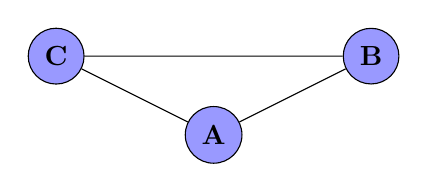
\begin{tikzpicture}
	  	\node[draw,circle,fill=blue!40!white](a) at (0,1) {\textbf{A}};
	  	\node[draw,circle,fill=blue!40!white](b) at (2,2) {\textbf{B}};
	  	\node[draw,circle,fill=blue!40!white](c) at (-2,2) {\textbf{C}};
	  	\draw (a)--(b) (b)--(c) (c)--(a);
  	\end{tikzpicture}
\end{document}